\chapter{Research Methodology}
%\label{chapter:Research Methodology}
\emph{The research methodology describes a chronological order of methodologies used to execute research. Components are research philosophy and approach, research design, data collection and preparation, data-driven sparse-sensing techniques and QR-based algorithm, and a case study in which two study areas are discussed.}

\section{Research philosophy and approach}

Within this research study, a positivism research philosophy is adopted. Positivism can be illustrated as a scientific conception to which a phenomenon can be known through empirical data based on natural processes. The concept relies on quantitative measurements and methods to illustrate the hydrological phenomenon and predict it in this way. As stated by Kabo et al. (2023), a mathematical model of hydrological flow is based on a positivist paradigm through which the natural world can be explained. According to Jansen (2023), a research methodology with a positivist perspective can only acquire data through measurements and observations. Data used in this research study is acquired through manual and sensor measurements of monitoring wells inherited by the City of Rotterdam. Next to the research philosophy, the research approach that is planned to be adopted is a quantitative research method. This research method involves the collection and analysis of numerical data to test hypotheses, examine patterns, and establish relationships between variables. The objective is to quantify and generalize findings. A quantitative research method uses a deductive approach, meaning a clear theory or hypothesis has to be researched. Consequently, the theory or hypothesis is tested, using specific observations or data. The research approach uses a top-down approach, meaning the theory or hypothesis that is available is first assessed instead of assessing data or observations (Jansen, 2023).

\section{Research design}
Following with the research design. The research design of this study describes the overall plan and guides the research study based on the objective. The research study has the purpose to generate a generic model in order to examine the degree of optimization of the GWMN of Rotterdam's municipal area. The approach employs a two-part research design:

\subsection{Descriptive design}
The initial phase aims to characterize the present state of the system, utilizing hydrogeological and geographical data of the research areas. The system description involves analyzing the distribution and coverage of monitoring wells in the municipality without manipulating variables. The descriptive design develops a detailed visualization of the existing GWMN, including parameters as distribution, coverage density, and groundwater level measurements.

\subsection{Quasi-experimental design}
The second phase includes an approach that manipulates the GWMN by simulating data and removing monitoring wells. These actions have the purpose to observe changes regarding network optimization. Initially, the research study includes 14 city districts and 4 industrial areas, however, a generic model is set-up. Only two specific research areas are included in the chapters “Research Methodology” and “Results”. The choice of the two specific research areas is based on factors such as measurement type, monitoring frequency, data availability, and density of the coverage area. Data loggers ensure that inaccessible and vulnerable locations within the city districts still can be frequently monitored through this approach. Certain monitoring wells are on inaccessible locations within the municipal area, however, through the use of data loggers these locations can still be actively monitored. The design continues with a quantitative method to analyze the impact of changes regarding monitoring network optimization, as reduction, over a longitudinal period.

\section{Data collection and preparation}
Within this research study, the time period includes 01-01-2010 to 01-01-2024. From 2010 to 2014, groundwater data was collected by the Gemeente Rotterdam. Field service employees of the field measurement service collected data through manual measurements. The measurements have taken place at the end of the month, trying to sample every four weeks and taking into account personal circumstances of the field employees. In the period of 2014-2018, however, the field measurements were carried out by an external contracting company. The transition to different field service employees in the year 2014 and 2018 possibly ensured errors and differences in the approach of data collection. From 2019 on, groundwater data will be collected by Gemeente Rotterdam again. This also means that multiple monitoring wells are transferred to data loggers instead of the manual collection method. Because of this transition, inaccessible locations were still monitored and data is collected more frequently, per day instead of per month.

\subsection{QGIS and PROWAT}
Starting with the first step of the data collection, the open-source QGIS and Sensor Management application of the Gemeente Rotterdam allow the availability of monitoring data for all unique monitoring wells within the municipal area. In QGIS, study areas of preference can be selected and transferred to the PROWAT system. PROWAT allows the data to be converted to an Excel data file. After which, data can be imported in the machine learning program Python.

\subsection{Pastas time series modeling}
The quasi-experimental research design starts with Pastas, a Python package made to analyze a sequence of data points that are collected over specific intervals of time (Artesia, n.d.). Data gaps are present in the dataset, resulting in potential problems later on in the development of the model. At first, a basic model is generated to visualize a simple time series model to simulate groundwater levels.

\subsubsection{Dependent time series}
A time series of groundwater levels is imported through the Pandas package. The dependent time series data describes the observed time series monitored by the municipality. The figure describes the groundwater level [m MSL] over a period of 01.01.2010 to 01.01.2024. Unique monitoring wells of the neighborhoods Rozenburg and Heijplaat are visualized. It is the intention that seasonal fluctuations and variabilities can be visualized in a plot. 

\subsubsection{Independent time series}
Continuing with importing the independent time series from an external dataset. In order to import the independent time series, two explanatory series are implemented. Precipitation and potential evaporation are the explanatory series. With use of precipitation and potential evaporation data, recharge to the groundwater can be calculated. The precipitation and evaporation data is conducted by the Royal Netherlands Meteorological Institute (KNMI) at weather station 344 in Rotterdam. The resulting figure describes the recharge level [m/day] over a time period of 01-01-2010 to 01-01-2024.

\subsubsection{Time series model}
After the dependent time series (based on observed GWL data) and independent time series (based on precipitation and evaporation data) are developed and plotted, the actual time series model is created. The dependent and independent time series are imported to the actual time series model. The imported time series are approved for missing values or inconsistencies in data. The model is solved through assessing optimal model parameters. The solution of the calculation can be plotted in a time series plot. The plot describes the observed data as a scatter plot and the simulation data, according to the independent data in a line plot. The actual time series model includes "Stress Model 1".

The observed data translates the groundwater level [m MSL] over a time period of 01-01-2010 to 01-01-2024. Besides the time series plot of the calculation, it is possible to accommodate an overview of the model. In the overview plot, the previous figure is plotted as well as a subplot of the residuals and noise, recharge and stresses, model parameters, and confidence interval. 

\subsubsection{Statistical substantiation}
Next to that, a summary of the developed performance metrics are shown in a table overview. The performance of the models is visualized through a bar plot. Performance metrics regarding the RMSE, R2, and EPV are shown. Nevertheless, based on the statistical data only, it can not be proved that a model is performing "good" or "bad". Therefore, additional statistical tests are executed. The Welch's t-test compares two data groups, "datalogger" and "manual measurement", within the dataset. The t-test is carried out to criticize whether a dataset with a combination of measurement types: datalogger, manual or a combination of both of them is recommended to be used. Nonetheless, in the context of environmental sciences, looking beyond statistical significance is key. Other factors such as reliability and data quality, confidence intervals, and the preference of stakeholders for example can shape the final decision regarding the choice of the data group. Overall, it is fundamental to consider a holistic approach that includes more factors besides statistical significance. Consequently, the decision is made to continue the research study with use of the data group "datalogger". The observed and simulated data of the measurement type "datalogger" are merged into a new data frame that is used in the next step "QR Factorization". 

\section{QR Factorization}
A data-driven algorithm is designed to optimize groundwater monitoring networks by determining the optimal number and location of monitoring wells for temporal and spatial level reconstruction. The algorithm can be explained by the dependency of data in order to make a certain decision, prediction or optimization process. Existing data from the municipality is used to study patterns, trends, and relationships between parameters. The method was first obtained by Ohmer et al. (2022) at the KIT and applied the methodology to a study area in Germany. The approach is included in the optimization approach regarding the municipality of Rotterdam. The network reduction method is utilized on the GWMN, using one-dimensional hydrograph data. The main process of the algorithm is the use of QR factorization, a mathematical approach that breaks down matrix A into the product of two matrices: Q and R. Q is an orthogonal matrix that transforms the original dataset into a new dataset with independent columns. This is essential for evaluating the unique contribution of each monitoring well. On the other hand, R is a triangular matrix, where values below the diagonal are equal to zero. The triangular matrix serves to rank monitoring wells based on their informational relevance. Figure 4.1, visualizes the decomposition of product A into matrices Q and R. 

\begin{figure}[htbp]
    \centering
    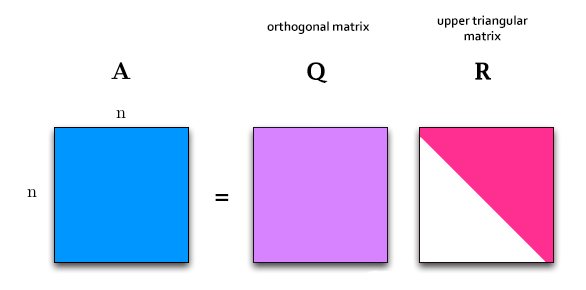
\includegraphics[width=0.40\linewidth]{figures/figures theory/qr rank.png}
    \caption{QR decomposition process from product A into matrices Q and R.}
\end{figure}

The optimization approach enables the network to be reduced along the Pareto front, balancing information loss against cost savings. To achieve the most accurate reconstruction with the least number of monitoring wells, the algorithm tests various reduction scenarios (25-50-75-90 percent) to identify the lowest reconstruction error for the monitoring network. It can, however, be possible that the optimal reduction percentage differs between the study areas. A reduction percentage of at least 25 percent should be applied to describe the system dynamics in the study areas, while a reduction percentage exceeding 75 percent would influence the accuracy of the reduction results, states Ohmer et al. (2022). 

Appendix B describes a detailed script regarding the QR factorization method. The Python package "PySensors" contains a data-driven algorithm for sparse sensor selection and signal reconstruction with dimensional reduction.

\section{Data analysis}
In terms of data analysis, the study is divided into two components:

\subsubsection{Descriptive design}
The purpose is to analyze the current conditions of the municipal area. This includes hydrogeological and geographical system descriptions of the municipal area as well as the study area. Based on the surface area of the chosen study areas, public spaces and the number of monitoring wells, the ratio of coverage can be calculated and analyzed.

\subsubsection{Quasi-experimental design}
A quasi-experimental design is employed to critically examine and compare data that is derived from automated data loggers and the manual collection method within the Gemeente Rotterdam. The analysis starts by determining the distinctiveness of the data groups within the dataset. This is done by a Welch’s t-test, a tool to ensure the distinctiveness of the data set corresponds to the automated and manual data collection methods. This first step is of major importance, since it is the substantiation of the data collection method that is chosen to continue the research with. 

The dataset undergoes a preprocessing phase, which involves a normalization and standardization process. In this phase, the mean, maximum, and minimum groundwater values are normalized and standardized across global and local scales. The preprocessing phase plays a major role, since it provides compatibility with the chosen modeling techniques. Furthermore, a division is made into a training (80\%) and test (20\%) dataset, designed to test the predictiveness and sensitivity of the model. The QR decomposition method is applied to the training data. This offers insight into the impact of different data collection strategies on model performance. 

Based on the informational relevance of the monitoring wells in the study areas, a hierarchical list can be generated. The hierarchical list applies a quasi-experimental evaluation of the impact of well reduction on the overall model performance. A systematic reduction (25-50-75-90 \%) of the network and the use of performance metrics, enables to assess the equilibrium between groundwater monitoring network reduction and accuracy of the model. This way, it is possible to gain understanding of different data collection methods and how they affect the robustness and accuracy of groundwater level predictions. The reduction approach continues with the selection of eliminated wells, the results are visualized in hydrographs. The hydrographs evaluate the performance of the monitoring wells based on their mean absolute error or also called the elimination error. This will provide an understanding of the informational relevance to the observed and reconstructed data. 

Through the application of the quasi-experimental methodology, the design ensures a comparative analysis of the data loggers and manual collection method.The methodology provides the effects and impact of the methods on model performance. 

\section{Case study}
The decision to examine Rozenburg and Heijplaat as case studies is based on the availability of data and the type of data collection method. Rozenburg and Heijplaat are relatively recently included in the municipal area. Comparing two distinct, but also very similar areas: high concentration of data loggers and a vast historical database facilitates an in-depth analysis of optimization levels. Additionally, this analysis could provide crucial insights into the modeling methodology.\\
\\
\subsection{Rozenburg}
The headland Rozenburg is notable for its eponymous village. Part of the headland has undergone extensive excavation measures and now serves the purpose of industrial landscape. Prior to 2010, the village maintained its autonomy as the municipality of Rozenburg, but eventually merged into the larger Gemeente Rotterdam. Positioned on the headland, the village finds itself in the inner dike area, enclosed by the industrial zones of Botlek and Europoort. The worlds of port and industrial activities, as well as nature, coexist. Therefore, part of the headland is called the “Groene Gordel” (green belt). In the 1950s, the headland primarily functioned as an agricultural area with a dune and nature reserve “de Grote Beer” on the western side. However, in the 1960s, major excavation measures took place to accommodate the development of Maasvlakte and Europoort industrial areas. Given its location, Rozenburg faces a notable risk for flood events. Consequently, infrastructure and port related activities in the area are situated at an average ground level of +5.7 meters MSL. The strategic elevation reduces the village’s vulnerability to potential flooding, particularly from the canal “Nieuwe Waterweg” (New Waterway) on the northern side of the district.\\
\\
Regarding the geology of the area, the first 22.91 meters are a Holocene formation that consists of sandy clay, medium-fine sand, clay, peat, and coarse sand. The presence of these sediments suggests a varied deposition environment; fluvial and marine processes. The diverse grain sizes of the sediment and the presence of an organic peat layer could indicate that infiltration rates can be varyinging and thus affect groundwater recharge and storage. Underneath the Holocene layer, a 1.46 meters thick layer of the formation of Kreftenheye is present. The formation consists of medium-coarse sand, little sandy clay, fine sand and cobbles with traces of clay and peat, see figure 4.1. An explaining legend is shown in figure 4.2. The composition of the second formation indicates a more permeable layer, in comparison with the top Holocene formation. This can also be explained by larger grain sizes, which allows for groundwater movement and possible occurrence of an aquifer. \\
\\
Collectively, the upper Holocene formation introduces a varied texture, ensuring heterogeneous permeability that affects groundwater flow and storage. The heterogeneity arose from the varied sediment composition, impacting the infiltration rate and groundwater dynamics. On the other hand, the Kreftenheye formation characterizes itself as a permeable formation, which is the result of the medium-coarse sand and cobbles. Given the focus of the research study on phreatic monitoring wells, the Holocene formation is only considered.\\
\\
\begin{figure}[h]
    \centering
    \begin{minipage}{0.30\linewidth}
        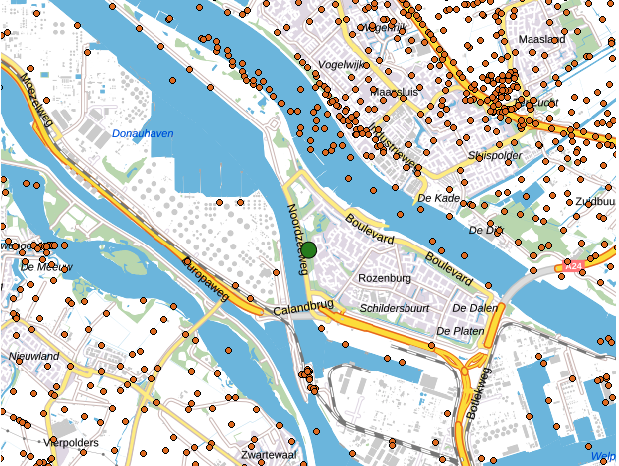
\includegraphics[width=\linewidth]{figures/roz/boor.png}
        \caption{Profile of geological formations and interpretation of formations of Rozenburg. Coordinates of the site of the drill profile are (x: 75250, y: 436180 (DINOloket, 2023).}
    \end{minipage}
    \hfill
    \begin{minipage}{0.60\linewidth}
        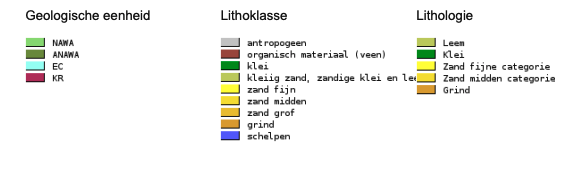
\includegraphics[width=\linewidth]{figures/roz/litho.png}
        \caption{Legend of the geological units and lithological classifications (DINOloket, 2023).}
    \end{minipage}
\end{figure}\\
\\
The location of the exact drill profile is shown in figure X. As can be seen in the figure, the location is in the southwestern side of the neighborhood, close to the connecting road. 
\\
\begin{figure}[htbp]
    \centering
    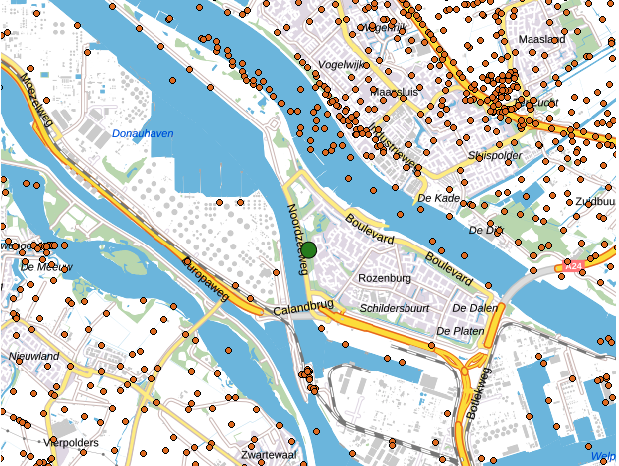
\includegraphics[width=0.60\linewidth]{figures/roz/drillsite.png}
    \caption{Exact location of the drill profile. Coordinates of the site of the drill profile are (x: 75250, y: 436180) (DINOloket, 2023).}
\end{figure}
\\
Rozenburg spans a total surface area of 411 hectares, with 324 hectares constituting land. The focus of Gemeente Rotterdam is on public terrains, monitoring wells located on private properties are excluded from consideration. Out of the 324 hectares of land, 1576 m2 are designated as public terrain. In the neighborhood of Rozenburg, 29 phreatic monitoring wells are present, which translates to 1 monitoring well for every  54.34 m2 of public terrain. A geographical representation of the neighborhood of Rozenburg is visualized in the figure. The blue markers highlight the locations of the monitoring wells, illustrating the distribution across the neighborhood.

\begin{figure}[htbp]
    \centering
    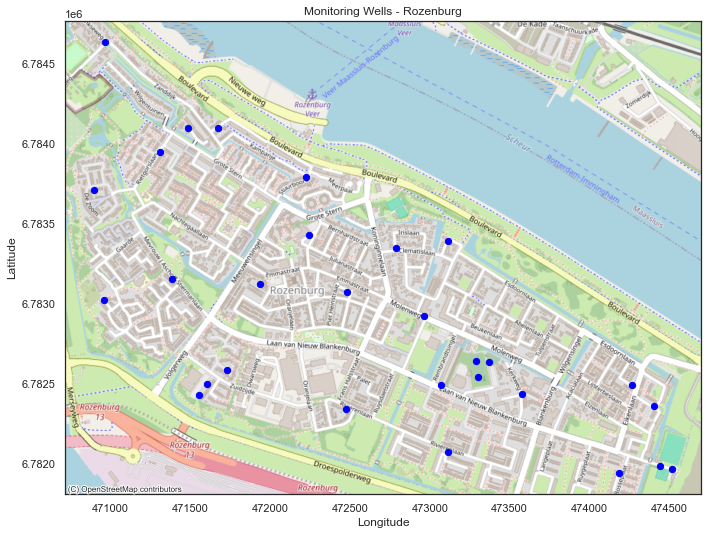
\includegraphics[width=0.55\linewidth]{figures/roz/basic_roz.png}
    \caption{Distribution of monitoring wells or also called the groundwater monitoring network of Rozenburg (Author's own contribution).}
\end{figure}

\newpage

\subsection{Heijplaat}
Since the mid-15th century, the hamlet "de Heij '' has been located at the northern side of the neighborhood "Charlois". At the north of the hamlet, the creek "de Koedood'' flew into the Meuse. However, years later, an industrial area called "de Heijsehaven'' was constructed at that site, where an artificial sand formation was formed as well. Only at the beginning of the 20th century, the idea of the garden village arose. Throughout the years, the village became more isolated because of the extension of the industrial areas. Figure X shows that Heijplaat is still surrounded by industrial areas and water outside the dike ring. Access to Heijplaat is solely possible through one entrance road, the Waalhavenweg. At the end of 2023, it emerged that the neighborhood experienced issues with the establishment of a new waste management firm. Additionally, water-related problems have been documented in the historic center as well. Construction initiatives have been proposed to address these issues with a focus on replacing the sewage system as a solution to the water-related inconveniences (DCMR, 2023). 

\begin{figure}[htbp]
    \centering
    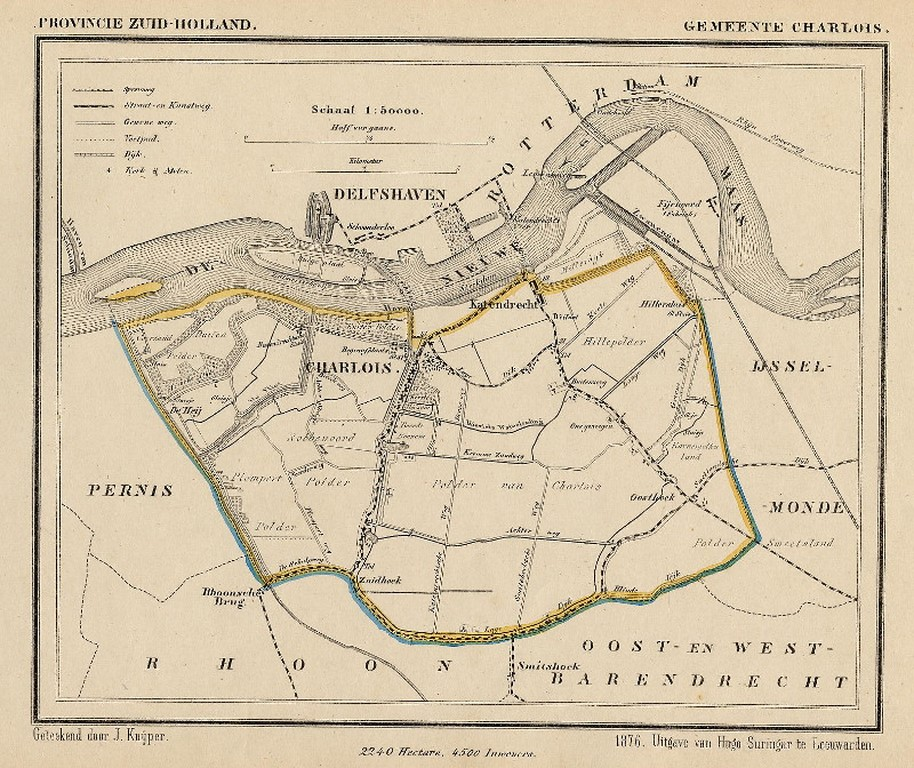
\includegraphics[width=0.60\linewidth]{figures/heij/charloisdeheij.jpeg}
    \caption{Geographical representation of the former hamlets: Charlois, Pernis, and the Heij (Suringar, 1867).}
\end{figure}

Figure X describes the lithology of Heijplaat. The subsurface in the eastern part consists of deposits from the formations Dunkirk III, Dunkirk I, and peat. A stratified geology is suggested with peat deposits present in areas with a high organic content. The peat deposits could influence water retention and filtration properties. On the western part of Heijplaat, however, the subsurface is characterized by the Dunkirk III formation atop a peat layer. The underlayer of peat indicates wet conditions in the past, which could influence the groundwater dynamics with layers of varying hydraulic properties. In the period of the 10th and 12th century, the peat landscape has been drained, which altered the landscape significantly. This showed itself through ground level reductions, necessitating dike construction. The manipulation of the landscape impacted and reshaped the groundwater recharge, flow and storage ability in the area. Overall, the area is marked by historical land alterations and complex, stratified geology, which influence the groundwater recharge, flow, and storage capacity in the neighborhood of Heijplaat. 

\newpage
\begin{figure}[htbp]
    \centering
    \begin{minipage}{0.45\linewidth}
        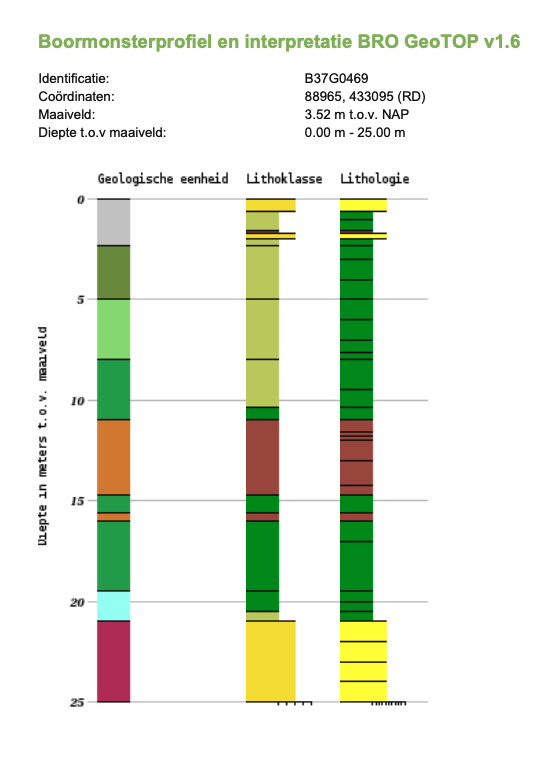
\includegraphics[width=\linewidth]{figures/heij/drillsite.png}
        \caption{Profile of geological formations and interpretation of formations of Heijplaat. Coordinates of the site of the drill profile are x, y: 88529, 433870 (DINOloket, 2023).}
    \end{minipage}
    \hfill
    \begin{minipage}{0.50\linewidth}
        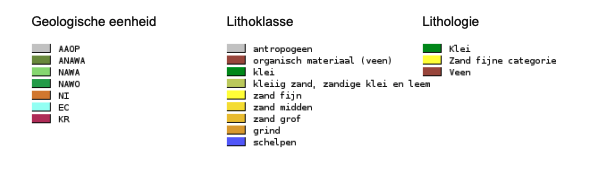
\includegraphics[width=\linewidth]{figures/heij/litho.png}
        \caption{Legend of the geological units and lithological classifications (DINOloket, 2023).}
    \end{minipage}
\end{figure}

\begin{figure}[htbp]
    \centering
    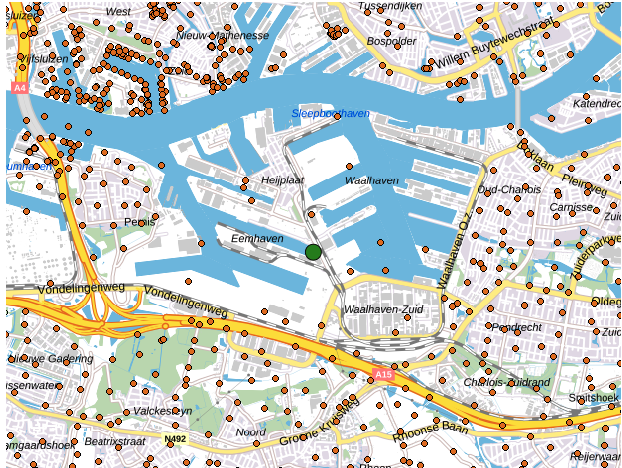
\includegraphics[width=0.40\linewidth]{figures/heij/boor.png}
    \caption{Exact location of the drill profile. Coordinates of the site of the drill profile are x, y: 88529, 433870 (DINOloket, 2023).}
\end{figure}

Heijplaat spans a total surface area of 39 hectares, all of which is land. Within the neighborhood, only 157 m2 are designated public terrain. The distribution of the monitoring wells over the neighborhood results in the presence of 1 monitoring well for every 11.21 m2. Figure X, offers a geographical representation of Heijplaat, which is part of the neighborhood Charlois. The blue marked points are representing the 14 locations of the phreatic monitoring wells within the neighborhood. 

\begin{figure}[h]
    \centering
    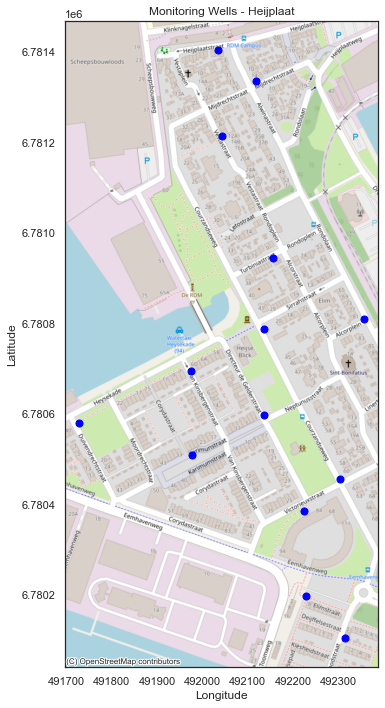
\includegraphics[width=0.70\linewidth]{figures/heij/basicheij.png}
    \caption{Distribution of monitoring wells or also called the groundwater monitoring network of Heijplaat (Author's own contribution).}
\end{figure}










